The first step in planet formation is accretion of planetesimals.  If accretion results in sufficient mass and energy to melt the initial body, all planetary bodies will differentiate into at least three compositional layers:  the dense core at the center, an intermediate density mantle, and a buoyant crust at the surface \citep{Elkins-Tanton2011a}.  The precise thickness of these layers and details such as the state (molten and/or solid) of the core, the temperature of mantle, and any layering in the crust, contain important information about the processes that shape the overall evolution of a planet \citep{Mocquet2011}.  Processes such as magma ocean formation and overturn, convective style and lithospheric mobility all shape interior structure and thermal evolution.  Global overturn models also make predictions about final crustal thickness.  The key variables in models of crust formed via accumulation of melt products above a convecting mantle predict a large range of crustal thickness.  The modeled production of crust via pressure release melting in a convecting mantle is strong function of temperature and volatile content.   If present on early Mars, plate tectonics would have cooled Mars more rapidly than stagnant lid convection. The thickness and state of the mantle and core affect the geometry and heat loss rate of convection, and thus the history of volcanism and volatile outgassing.

The intermediate size of Mars between Earth and the Moon, the only two bodies for which seismic and heat flow data have been acquired to date, places it in the sweet spot for understanding early planetary formation. The Moon's diameter limits the phase transitions in the interior to those occurring at relative shallow depths on Earth \citep{Khan_etal13, Kuskov2014}, thus limiting applicability to larger bodies. Mars is large enough to be in the same pressure regime as Earth’s upper mantle, small enough to be geologically arrested enough to preserve its original crust.  Mars’ relatively small volume also means that it contains insufficient heat producing elements to maintain vigorous present day geologic activity, thus preserving much of its original crust. Additionally, there is a wealth of data for Mars, including from both missions and meteorites, that provide strong constraints on its original composition and geologic evolution. 
\begin{figure}[h!]
\begin{center}
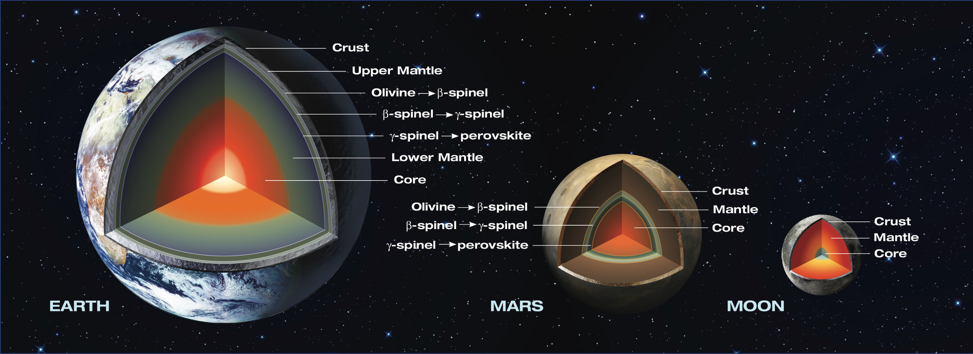
\includegraphics[width=0.95\textwidth]
{figures/Fig1_1.png}
\caption{Interior structure of Earth, Mars and the Moon, with known phase transitions for Earth and possible phase transition locations for Mars.}
\label{fig:Fig1_1.png} 
\end{center}
\end{figure}

The InSight mission will provide the first seismic and heat flow data for Mars, enabling unprecedented constraints on interior structure and evolution.  InSight launches in May of 2018, and arrives at Mars on November 26, 2018, landing on Elysium Planitia \citep{Golombek2017}.  The three primary instruments are the Seismic Experiment for Interior Structure (SEIS), the Heat Flow and Physical Properties Package (HP$^3$), and the Rotation and Interior Structure Experiment (RISE).   SEIS consists of a set of 3 very broad band seismometers coupled with 3 short period seismometers \citep{Lognonne2018}. Techniques for determining interior structure with a single station are described in \citet{PANNING2015,BOSE2017}. HP$^3$ is a self-hammering mole that deploys a tether with embedded temperature sensors to a depth of 3-5 m, taking thermal conductivity measurements as it descends \citep{Spohn2018}.  RISE \citep{Folkner2018} uses two low gain X-band antennas to precisely track the lander location over a Martian year to determine the rotation of Mars, as well as its precession and nutation. RISE data will enable the first estimate of Mars’ nutation, thus providing tight constraints on core size, density and state (liquid versus solid).  The lander Instrument Deployment Arm \citep{Trebi-Ollennu2018} will deploy SEIS and HP$^3$ on the surface of Mars, with the aid of two cameras to image the deployment zone \citep{Maki2018}.  Additionally, a pressure sensor, wind sensors, and a magnetometer are used to decorrelate seismic events from atmospheric effects or lander magnetic field variations (Banfield et al., 2018). The HP$^3$ experiment includes a radiometer to determine surface temperature variations \citep{Spohn2018}. Finally, color images of the surface as well as experiments with the arm and scoop coupled with information from SEIS and HP will be used to better understand the geology and physical properties of the surface and shallow subsurface \citep{Golombek2018}


Using data from its three primary instruments, InSight will accomplish six science objectives \citep{Banerdt2013}:
\begin{itemize}
\item Determine the size, composition and physical state of the core
	\item Determine the thickness and structure of the crust
	\item Determine the composition and structure of the mantle
	\item Determine the thermal state of the interior
	\item Measure the rate and distribution of internal seismic activity
\item Measure the rate of impacts on the surface
\end{itemize}

In this paper, we will begin by summarizing the available constraints on the interior of Mars.  We then describe the theoretical framework for models of the interior structure and thermal evolution including equations of state, convection models, and their interdependence. Finally, we describe an approach to integrating the new constraints to be provided by InSight into a new framework for understanding early differentiation, core formation, dynamo history, mantle mineralogy and volatile content, thermal evolution including dynamo history, and crustal formation processes. 

